\subsection{A short trip to Finite Elements Analysis (FEA)}
To calculate deformations and stresses of structures, \begriff{finite element analysis} is an important and often used method. It divides the structure in several points, calles \begriff{nodes}, and \begriff{elements} between those nodes. 
\bigskip

As the finite element analysis divides a part in very many elements and there are a lot of equations to solve for every node, the finite element analysis was not very popular until the 1950s. With the rise of the computer it was possible to solve thousands of equations in a few minutes. The more the computer was developed, the more programs for finite element analysis were developed.
\bigskip

In the following subsection I will give a short review about finite element analysis showing on the example of an one dimensional bar leading to methods of solving more complex problems of two- and three-dimensional problems.
\bigskip

Let us assume that the rod is on simple support and under a constant axial load of $q_0$, length $L$, Young's Module $E$ and cross-section area $A$:
\bigskip

\begin{figure}
\begin{center}
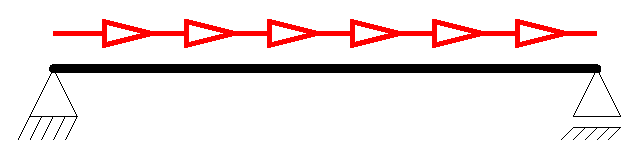
\includegraphics[scale=1]{figs/OneDimensionalBar}
\caption{One dimensional bar}
\end{center}
\end{figure}

\bigskip
From the elementary courses of mechanics we know that
\begin{align}
EA\,\frac{du}{dx}+q_0=0 \label{Rod_Main}
\end{align}
As we now proceed we can assume any trial function $û(x)$ that satisfies the boundary conditions that $û=0$ at $x=0$ and $\frac{dû}{dx}=0$ at $x=L$.

Let $û$ be a polynomial function of $x$ with 
\begin{align}
û(x)=c_0\,+\,c_1\,x\,+\,c_2\,x \nonumber
\end{align}
with the unknown constants $c_0$, $c_1$ and $c_2$. According to the boundary conditions we have $c_0=0$ and $c_1=-c_2\,L$. Now our trial function looks like
\begin{align}
û(x)=-2c_2Lx\,+\,c_2x=c_2(x\,-\,2Lx) \nonumber
\end{align}
As we substitute $û$ in eq.\ref{Rod_Main} we come to the following equation:
\begin{align}
2AEc_2+q_0=R_d \nonumber
\end{align}
with $R_d$ as the \begriff{residual}. We see that for $c_2=\frac{-q_0}{2AE}$ the residual is equal to zero on every point of the rod. We will see later, that this will not happen for every trial function. As the residual is equal to zero on every point our solution is equal to the exact solution:
\begin{align}
û(x)=(2xL-x^2)\frac{q_0}{2AE}=u(x) \nonumber
\end{align}
Assuming a different trial solution, e.g. $û(x)=c_0\,sin(\frac{\pi\,x}{2L})$, we see that the boundary conditions $û=0$ at $x=0$ and $\frac{dû}{dx}=0$ at $x=L$ are satisfied. As the equation has only one free parameter, $c_0$, it is called a \begriff{one-parameter solution}.

As we substitute $\frac{d^2û}{dx^2}$ again in eq.\ref{Rod_Main} we come to:
\begin{align}
-EA\, c_0\,sin\left(\frac{\pi\,x}{2L}\right)\frac{\pi^2}{4L^2}+q_0=R_d \nonumber
\end{align}

We see that there is no constant $c_0$ that makes $R_d$ equal to zero on every point of the rod. We can try to make $R_d$ equal to zero on one point (for example $x=0.5L$), but the errors would be quite huge. 

An opportunity to make the mistakes smaller is to add more parameters to our trial solution like
\begin{align}
û(x)=c_0\,sin\left(\frac{\pi\,x}{2L}\right)\,+\,c_1\,sin\left(\frac{3\,\pi\,x}{2l}\right)\,+\,c_2\,sin\left(\frac{5\,\pi\,x}{2L}\right)\,+... 
\end{align}
which decreases the mistake the more parameters we invent how fig.\ref{ExactVSParameter} shows. This technique is called the \begriff{point collocation technique}.

\bigskip
An other method is the \begriff{weighted residual technique}, where $W(x)$ is the \begriff{weighted function}. We will multiplicate the residual of our trial function with this weighted function and integrate it over the whole area. 
\begin{align}
\int\,W(x)\,R_d(x)\,dx=0 \nonumber
\end{align}
Theoretically we can chose every function as weighted function as long as they are integrable, but \eigenname{Galerkin} introduced the idea of letting $W(x)$ be $û(x)$ itself in 1915, which works pretty well with most problems (see fig.\ref{ExactVSGalerkin})

\bigskip
So for our problem with the one dimensional rod $W(x)$ will be
\begin{align}
W(x)=sin\left(\frac{\pi\,x}{2L}\right) \nonumber
\end{align}

And the integral would be
\begin{align}
\int\,sin\left(\frac{\pi\,x}{2L}\right)\,\left(-EA\, c_0\,sin\left(\frac{\pi\,x}{2L}\right)\frac{\pi^2}{4L^2}+q_0\right)\,dx=0 \nonumber
\end{align}
which will lead to
\begin{align}
c_0=\frac{16\,L^2q_0}{\pi^3EA} \nonumber
\end{align}
\bigskip

\begin{figure}[!h]
\begin{center}
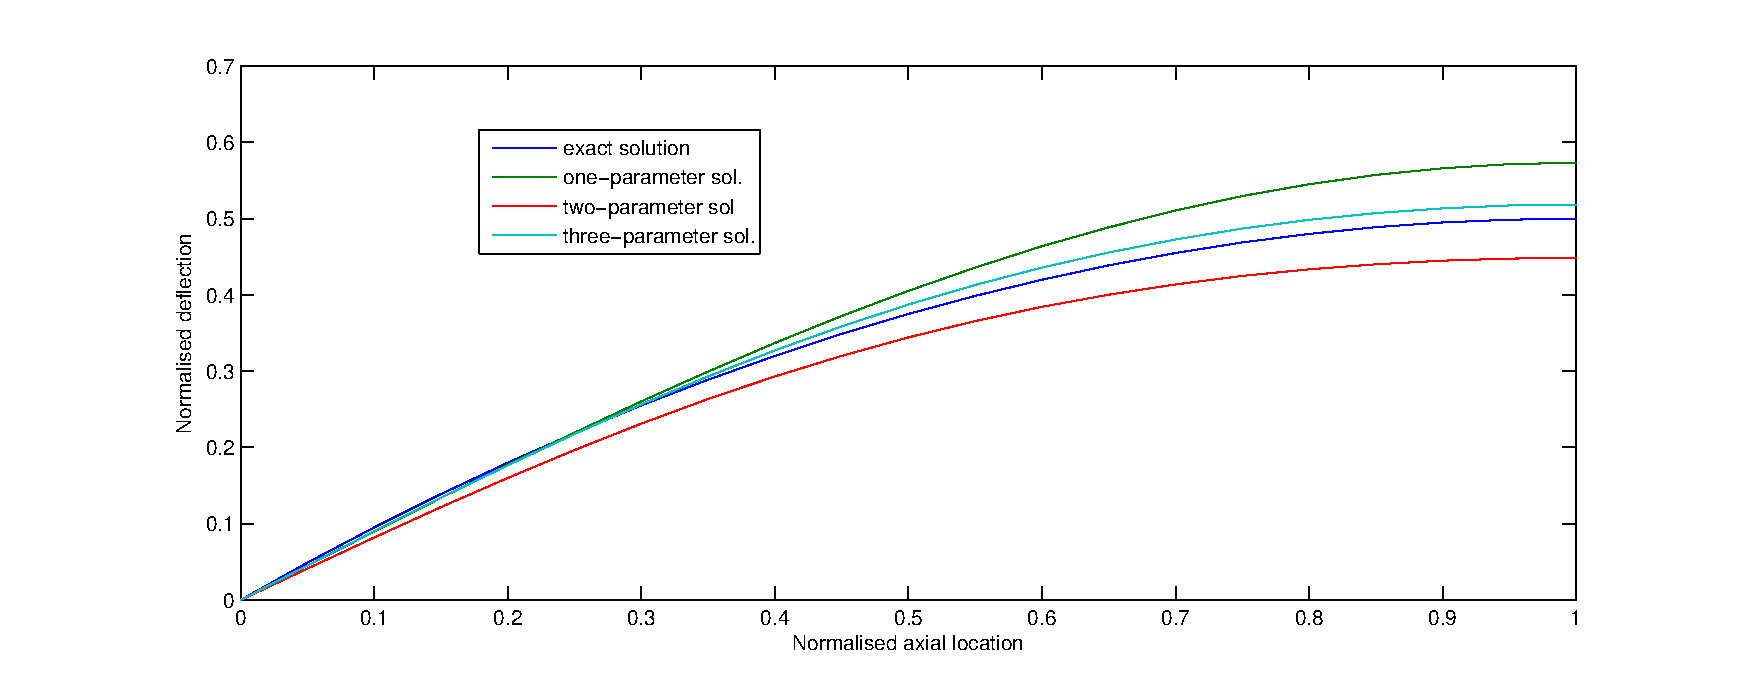
\includegraphics[scale=0.6]{figs/ExactVSParameter} 
\caption{The exact solution compared to the one-, two-, and three-parameter solution}
\label{ExactVSParameter}
\end{center}
\end{figure}
\begin{figure}[!h]
\begin{center}
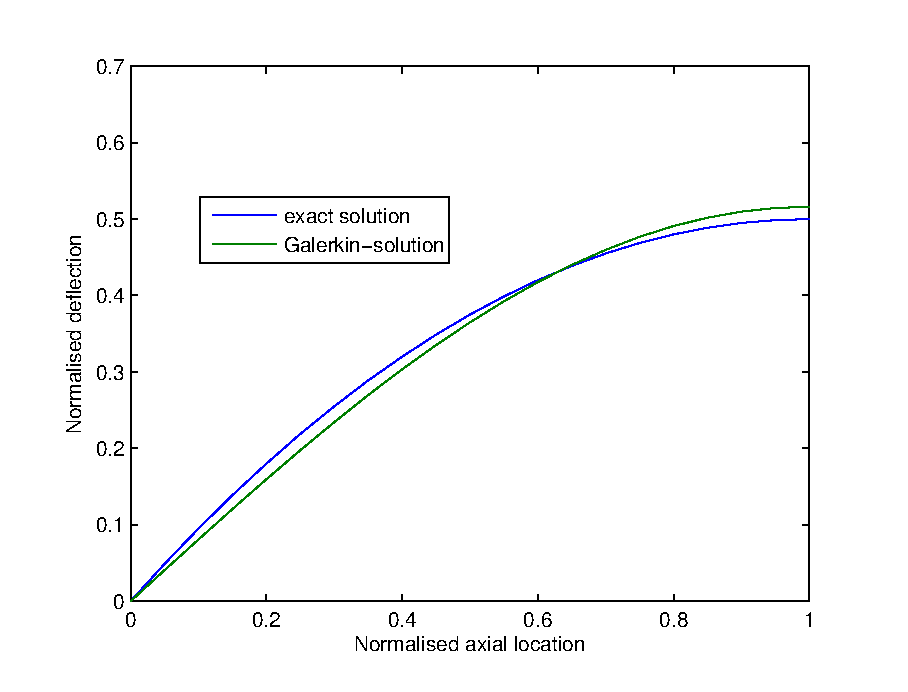
\includegraphics[scale=0.8]{figs/ExactVSGalerkin.eps} 
\caption{The exact solution compared to the solution with a \eigenname{Galerkin}-weighted function}
\label{ExactVSGalerkin}
\end{center}
\end{figure}

{\bf Note:} The \eigenname{Galerkin}-solution here is made for a one-parameter trial function. For a more-parameter trial function with $û(x)\,=\,\sum c_i\,û_i(x)$ there would be weighted functions $W_i$ that make the approximative solution even more exact
\bigskip 

\subsection{Basic methods of my FEA-program}
In the following I will derive the equations used in my one-dimensional finite element program, first for the static case and then, much more complicated, for the dynamic case. I will only give a very short overview of the theoretical basics of FEA, the interested reader is referred to \cite{seshu} and \cite{ramamurty}.

\bigskip
\bigskip


\begin{minipage}{\textwidth}
    \begin{minipage}[t]{0.5\textwidth}
     
     \paragraph{The Beam Element} Our one-dimensional beam element consists of two nodes at each end. Every node has two degrees of freedom as it can move normally to the beams axis and rotate around an axis normally to the grid. We define a vector $\vec{q}$  describing the deformations of one element and a vector $\vec{f}$ describing the forces and torques attached to the nodes:
    \end{minipage}
    \hfill
    %\mbox{\numexpr{0.95-#5}} geht vielleicht auch irgendwie
    \begin{minipage}[t]{0.5\textwidth}				%ehemals 0.45 [LARS]
      ~\\[-1ex]%fakezeile, um beide minipages mit der t-Zeile auszurichten
      \centerline{
      \psfrag {n1} {$n_1$}
      \psfrag{n2}{$n_2$}
      \psfrag{u1}{$u_1$}
      \psfrag{u2}{$u_2$}
      \psfrag{p1}{$\phi_1$}
      \psfrag{p2}{$\phi_2$}      
      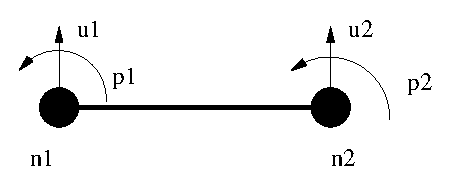
\includegraphics[scale=1]{figs/beamElement1.eps}}
    \end{minipage}
  \end{minipage}

\begin{align}
\vec{q}&=\left(\begin{array}{c}
u_1 \\ 
\phi_1 \\ 
u_2 \\ 
\phi_2
\end{array} \right)&\vec{f}=\left(\begin{array}{c}
F_1 \\ 
M_1 \\ 
F_2 \\ 
M_2
\end{array}\right)\nonumber
\end{align}
where $u_1$ and $\phi_1$ are the displacements and rotations of the first node, respectively, and  $u_2$ and $\phi_2$ for the second node in the same manner. $F_i$ and $M_i$ are for the force and torques at node $i$.
\bigskip 
\paragraph{The k-Matrix}

We now want to derive a matrix $\vec{k}$, so that $\vec{f}=\vec{k}*\vec{q}$. For that we will look at a beam, deformed in only one degree of freedom, based on the \begriff{Beam Theory} of \eigenname{Euler} and \eigenname{Bernoulli}. There are a whole bunch of books about the Beam Theory, the interested reader can read for example \cite{timoschenko}. For deriving the k-matrix we will deform our beam element four times, so it will just deform in one of the four degrees of freedom.\\
\bigskip
\begin{figure}
\begin{center}
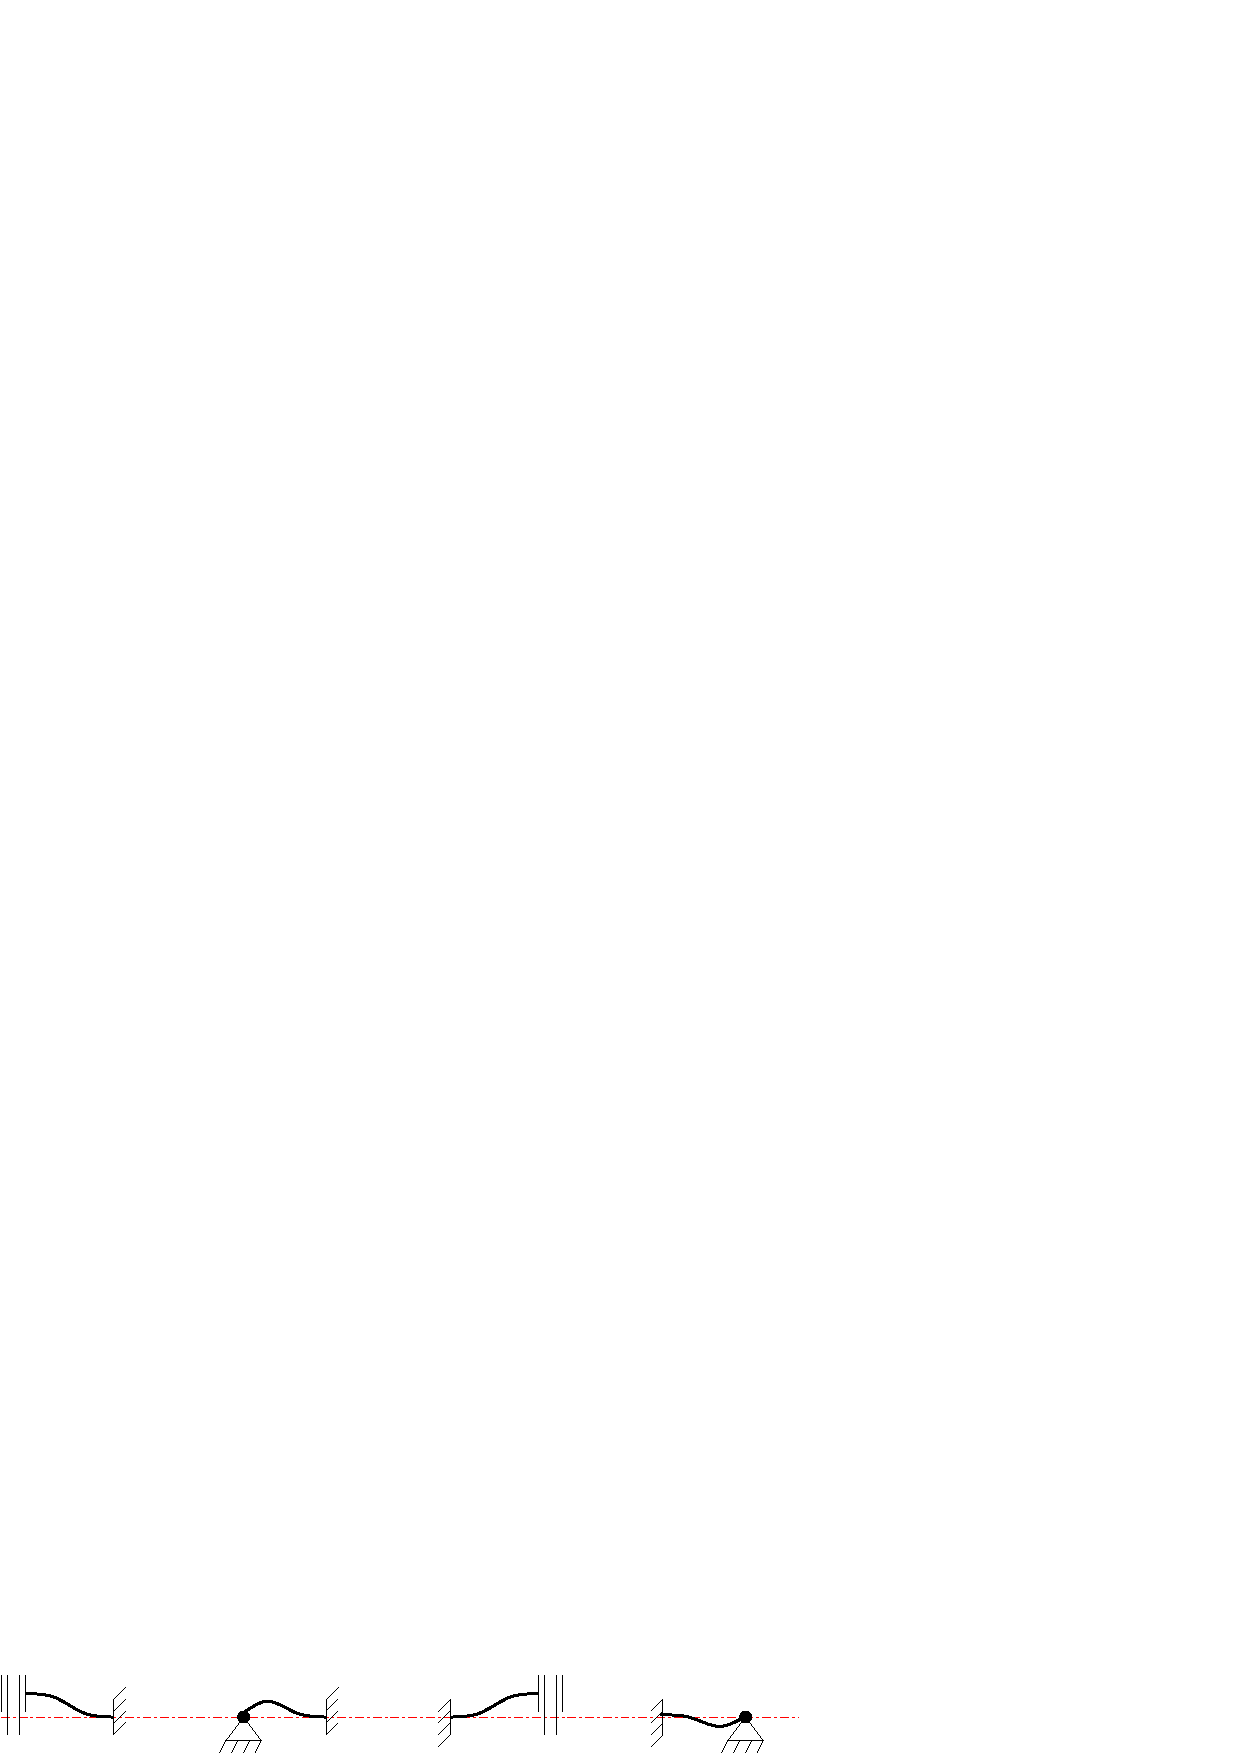
\includegraphics[scale=1.2]{figs/fourDeformations}
\caption{The four different basic deformations of a beam element}
\end{center}
\end{figure}
\bigskip 

\begin{minipage}{\textwidth}
    \begin{minipage}[t]{0.3\textwidth}
     
     For a beam of lenght $l$ I will demonstrate the derivation of the k-matrix on an example of a beam which has only a displacement in its first degree of freedom. I will use the Beam Theory of \eigenname{Euler} and \eigenname{Bernoulli} to calculate the needed forces and torques at each node.
    \end{minipage}
    \hfill
    %\mbox{\numexpr{0.95-#5}} geht vielleicht auch irgendwie
    \begin{minipage}[t]{0.7\textwidth}				%ehemals 0.45 [LARS]
      ~\\[-1ex]%fakezeile, um beide minipages mit der t-Zeile auszurichten
      \centerline{
      \psfrag{m1}{$M_1$}
      \psfrag{m2}{$M_2$}
      \psfrag{f1}{$F_1$}
      \psfrag{f2}{$F_2$}
      \psfrag{u1}{$u_1$}
      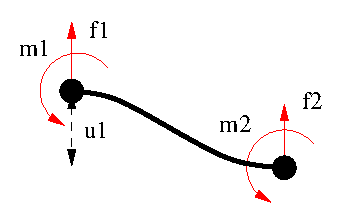
\includegraphics[scale=1.5]{figs/deformBar1.eps}}
    \end{minipage}
  \end{minipage}
  \bigskip
  
  The moment in the beam $M(x)$ for a $x$ running from left to right over the beam's axis is:
  \begin{align}
  M(x)=F_1\,x- M_1 \label{Momentenverlauf}
  \end{align}
  Integrating $EI\,w''=M(x)$ twice with \ref{Momentenverlauf} gives:
  \begin{align}
  w'&=\frac{1}{EI}\left(\frac{1}{2}F_1\,x^2-M_1\,x+C_1\right) \label{neigungslinie}\\
  w&=\frac{1}{EI}\left(\frac{1}{6}F_1\,x^3-\frac{1}{2}M_1\,x^2+c_1\,x+C_2\right) \label{biegelinie}
  \end{align}
  With the boundary conditions
  \begin{align}
  w(0)=u_1; && w'(0)=0; &&& w(l)=0; &&& w'(l)=0 \nonumber
  \end{align}
  inserted in \ref{biegelinie} and \ref{neigungslinie} we get the force-vector $\vec{f}=k_1*u_1$:
  \begin{align}
  \vec{f}=\frac{EI}{l^3}\left(\begin{array}{c}
  12 \\ 
  6\,l \\ 
  -12 \\ 
  6\,l
  \end{array} \right)\,u_1
  \end{align}
  Analogously we find $k_2$, $k_3$ and $k_4$ for deformation of an other degree of freedom. Because of Superposition we can write for $\vec{f}$ for deformation of all degrees of freedom just the sum of all deformations:
  \begin{align}
  \vec{f}&=\sum\,\vec{k_i}\,\vec{q_i} \nonumber \\
  \vec{f}&=\vec{k_1}\,\vec{q_1}+\vec{k_2}\,\vec{q_2}+\vec{k_3}\,\vec{q_3}+\vec{k_4}\,\vec{q_4} \nonumber \\
  \vec{f}&=\vec{k}\,\vec{q} \label{grundgleichung}
  \end{align}
  with
  \begin{align}
  \vec{k}=\left(\begin{array}{cccc}
  \vec{k_1} & \vec{k_2} & \vec{k_3} & \vec{k_4}
  \end{array} \right) \label{k-matrix}
  \end{align}
  For our one dimensional beam element we can derive $\vec{k}$ as:
  \begin{align}
  \vec{k}=\frac{EI}{l^3}\left[\begin{array}{cccc}
  12 & 6\,l & -12 & 6\,l \\ 
  6\,l & 4\,l^2 & -6\,l & 2\,l^2 \\ 
  -12 & -6 \,l & 12 & -6\,l^2 \\ 
  6\,l & 2\,l^2 & -6\,l^2 & 4\,l^2
  \end{array} \right] \label{beam-k-matrix}
  \end{align}
  \bigskip
  
  \paragraph{Shape Functions} In our model forces and torques can only be applied at the nodes, but unluckily in many cases forces and torques are acting somewhere between the nodes. For this reason you need shape functions defining which part of the force is acting on which node of the element. A shape functions of a node has the property that it will be 1 at that specific node and 0 on all other nodes, which is trivial, because forces acting on that node will act with 100\% on that node and forces acting on other nodes will not affect that node. Also the sum of all shape functions has to be 1 at every location of the body. I will show two different types of famous shape functions.
\bigskip

\begin{figure}[!h]
\begin{center}
\psfrag{n1}[m][m]{first node}
\psfrag{n2}[m][m]{second node}
\psfrag{l2}{$x=\frac{1}{2}l$}
\psfrag{1}{1}
\psfrag{0}{0}
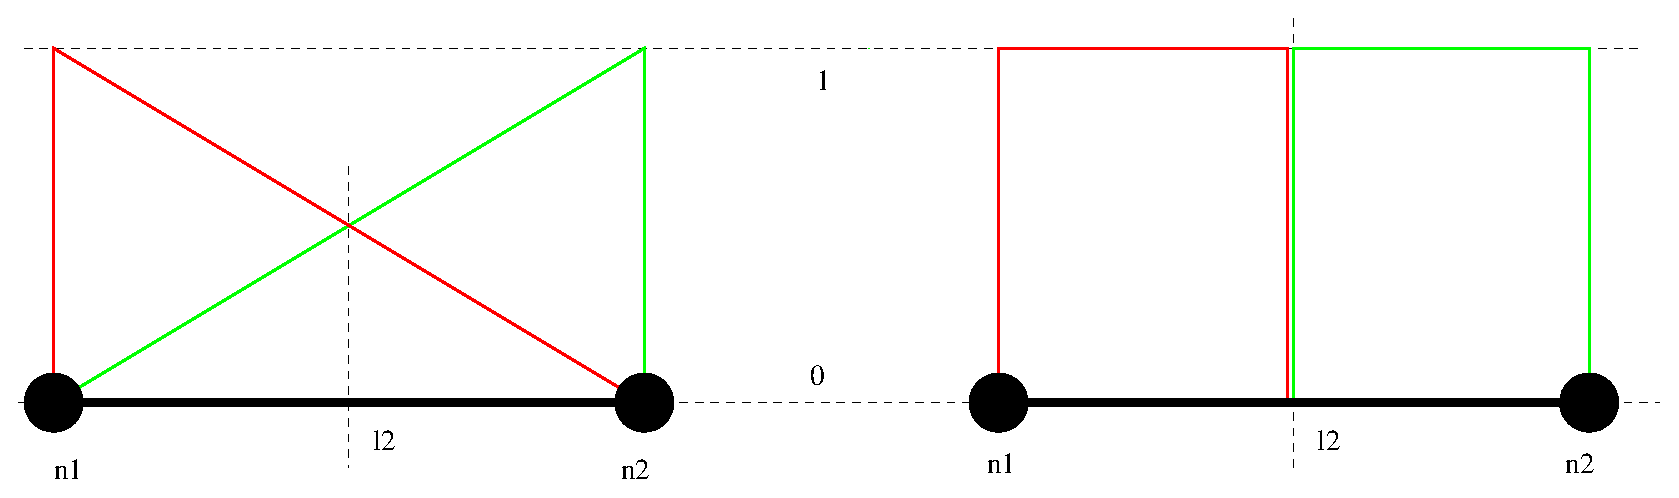
\includegraphics[scale=0.6]{figs/shapeFunctions} 
\caption{Visualisation of the linear and the plumbed one dimensional shape function}
\label{shapeFunctions}
\end{center}
\end{figure}
In the linear shape function you use a linear function $s_l(x)=1-\frac{x}{l}$ for the left node and $s_r(x)=\frac{x}{l}$ for the right node. The forces acting with this model on the left and right node are
\begin{align}
f_l=\int_0^lq(x)\,s_l(x)\,dx+\sum_iF_i\,s_l(x_i) \nonumber \\
f_r=\int_0^lq(x)\,s_r(x)\,dx+\sum_iF_i\,s_r(x_i) \nonumber
\end{align}
with $q(x)$ as a line force and $F_i$ as single forces. The same is also with torques.
\bigskip

An other advantage of this function is, that you can calculate the displacement on every point along the element using the shape functions with
\begin{align}
\vec{q(x)}=\vec{q_l}\,s_l(x)+\vec{q_r}\,s_r(x)
\end{align}
where $\vec{q_l}$ and $\vec{q_r}$ are the displacements at the left and right node.
\bigskip

The second method is simpler and is called the plumbed shape function. It is not that accurate like the linear shape function, but when using lots of elements or constant line forces (or slowly changing line forces) and single forces attached to the nodes it will not make any difference. Here you just attach all forces acting between the left node and the middle of the element to the left node and all forces acting between the middle of the element and the right node to the right node. So the forces attached to each node are given by
\begin{align}
f_l&=\int_0^{l/2}q(x)\,dx+\sum_iF_i &&0<x_i<l/2 \nonumber \\
f_l&=\int_{l/2}^{l}q(x)\,dx+\sum_iF_i &&l/2<x_i<l \nonumber
\end{align}
For the attached program \textbf{BEAM.m} I chose the plumbed shape function because it is simple to calculate and it will not give different results as I have a constant line force anyway.
\bigskip

\paragraph{Assembling a Problem} As you may have noticed, I used small letters for k-matrix as well as for f-, and q-vector. This should indicate that the matrix is just for one element. If you want to assemble a matrix for the whole system you need to add all the matrices in respect to their global and nodal counting system.
\bigskip 

\begin{figure}[!h]
\begin{center}
\psfrag{nodal degree of freedom}[m][m]{nodal degree of freedom}
\psfrag{global degree of freedom}[m][m]{global degree of freedom}
\psfrag{1, 2}{1, 2}
\psfrag{3, 4}{3, 4}
\psfrag{5, 6}{5, 6}
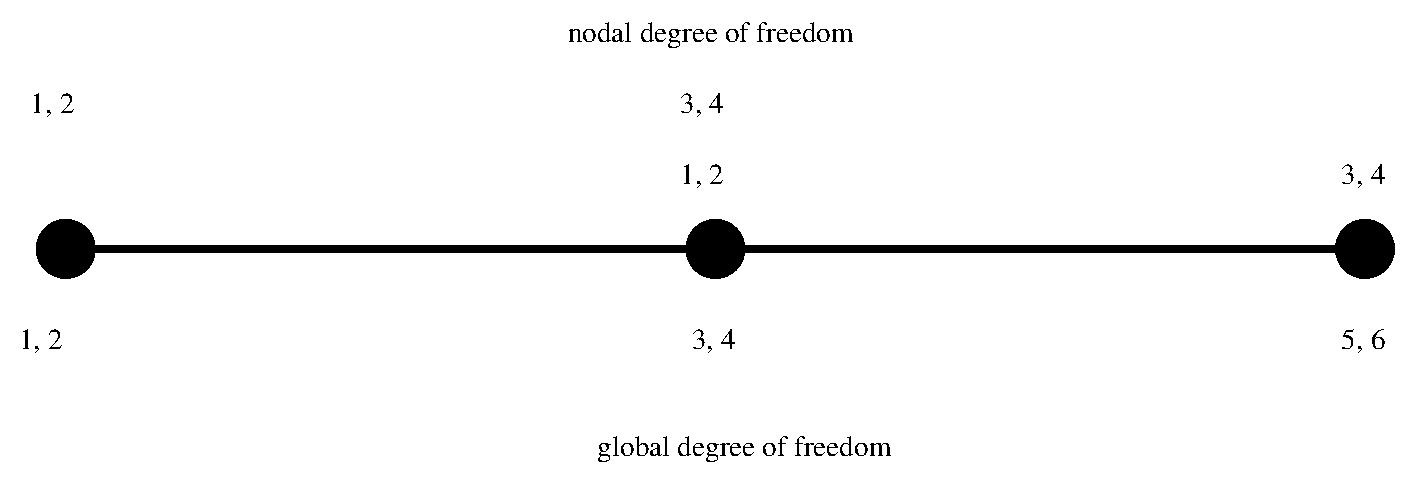
\includegraphics[scale=0.6]{figs/assembly} 
\caption{Assembly of two beam elements}
\label{assembly}
\end{center}
\end{figure}

As you can see in fig.\ref{assembly} every DOF has both a nodal number as well as a global number. 
